Le SIF de l'UM2 (ref.~\cite{GitLabSIF}) a mis a disposition des étudiants un service GitLab que nous avons utilisé. Git a été choisi comme gestionnaire de version car c’est celui utilisé par GitLab (ref.~\cite{GitLab}).
Git est un gestionnaire de version décentralisé, qui permet d'avoir accès à ceux-ci avec une simple connexion internet.
Il s'utilise avec des systèmes de branches et le plus souvent depuis un terminal, mais nous l'avons aussi utilisé avec Gitg, qui est une interface permettant d'avoir un visuel (cf.~\ref{gitg}).

\begin{figure}[h]
\caption{\label{gitg} Capture de Gitg}
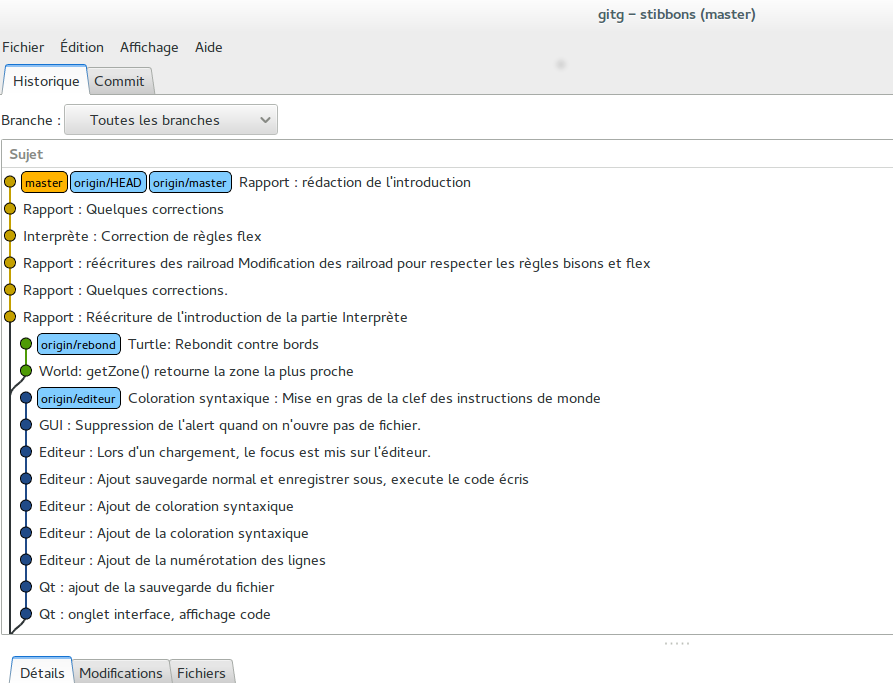
\includegraphics[scale=0.35]{doc/report/uml/gitbranche.png}
\end{figure}

Les commandes les plus utilisées sont les suivantes~:
\begin{description}
\item[git checkout nom-branche] permet de changer de branche~;
\item[git branch] permet de savoir sur quelle branche on est~;
\item[git add fichiers] permet de suivre des fichiers (enregistrer les modifications qu'on fait sur des fichiers)~;
\item[git commit] permet de sauvegarder des changements des fichiers~;
\end{description}

De plus, GitLab possède une traqueur de bug. Ce dernier permet d'ouvrir des «~issues~» qui peuvent être fermées, ré-ouvertees, commentées, etc.
